% ============================================================
%  MAIN THESIS FILE
%  Supply Chain Digital Twin using Reinforcement Learning
%  VNIT Nagpur -- B.Tech CSE Final Year Project 2025
% ============================================================
\documentclass[12pt, a4paper, oneside]{report}

% ---- Packages -----------------------------------------------
\usepackage[top=1in, bottom=1in, left=1.5in, right=1in]{geometry}
\usepackage{graphicx}
\usepackage{setspace}
\usepackage{times}            % Times New Roman font (standard for VNIT reports)
\usepackage{titlesec}
\usepackage{tocloft}
\usepackage{hyperref}
\usepackage{amsmath}
\usepackage{amssymb}
\usepackage{booktabs}
\usepackage{longtable}
\usepackage{array}
\usepackage{multirow}
\usepackage{caption}
\usepackage{subcaption}
\usepackage{fancyhdr}
\usepackage{indentfirst}
\usepackage{parskip}
\usepackage{xcolor}
\usepackage{listings}
\usepackage[backend=biber, style=ieee, sorting=none]{biblatex}
\addbibresource{references.bib}

% ---- Page Style ---------------------------------------------
\pagestyle{fancy}
\fancyhf{}
\fancyhead[R]{\small Supply Chain Digital Twin using RL}
\fancyhead[L]{\small VNIT Nagpur}
\fancyfoot[C]{\thepage}
\renewcommand{\headrulewidth}{0.4pt}

% ---- Chapter Heading Style (matches seniors' layout) --------
\titleformat{\chapter}[display]
  {\normalfont\large\bfseries\centering}
  {\chaptertitlename\ \thechapter}
  {10pt}
  {\Large}
\titlespacing{\chapter}{0pt}{-20pt}{20pt}

% ---- Line Spacing -------------------------------------------
\doublespacing

% ---- Document -----------------------------------------------
\begin{document}

% ============================================================
%  FRONT MATTER
% ============================================================
\pagenumbering{gobble}        % No page numbers on title pages

% ============================================================
%  TITLE PAGE  (matches VNIT seniors' format exactly)
% ============================================================
\begin{titlepage}
\centering

% University logo placeholder -- replace vnit_logo.png with actual file

\includegraphics[width=3.5cm]{images/vnit_logo.png}

\vspace{0.5cm}

{\Large \textbf{Supply Chain Digital Twin using Reinforcement Learning}}

\vspace{0.8cm}

{\normalsize Project report submitted to}\\[0.3cm]
{\normalsize Visvesvaraya National Institute of Technology, Nagpur in partial fulfillment of the}\\
{\normalsize requirements for the award of the degree}

\vspace{0.5cm}

{\large \textbf{Bachelor of Technology}}\\[0.2cm]
{\normalsize in}\\[0.2cm]
{\large \textbf{Computer Science and Engineering}}

\vspace{0.8cm}

{\normalsize by}

\vspace{0.5cm}

\begin{tabular}{c c}
    Ayaan Khan     & Arya Patil \\
    (BT22CSE001)   & (BT22CSE003) \\[0.4cm]
    Nihaal Badam   & Swastik Ankulge \\
    (BT22CSE004)   & (BT22CSE013) \\
\end{tabular}

\vspace{0.8cm}

{\normalsize under the guidance of}\\[0.4cm]
{\large \textbf{Dr. Ravindra B. Keskar}}

\vspace{0.8cm}

{\normalsize Department of Computer Science and Engineering}\\
{\normalsize Visvesvaraya National Institute of Technology}\\
{\normalsize Nagpur 440010 (India)}\\[0.4cm]
{\normalsize 2022 -- 2026}

\vfill
\end{titlepage}

% Second title page with copyright line (as in seniors' thesis)
\begin{titlepage}
\centering


\includegraphics[width=3.5cm]{images/vnit_logo.png}

\vspace{0.5cm}

{\Large \textbf{Supply Chain Digital Twin using Reinforcement Learning}}

\vspace{0.8cm}

{\normalsize Project report submitted to}\\[0.3cm]
{\normalsize Visvesvaraya National Institute of Technology, Nagpur in partial fulfillment of the}\\
{\normalsize requirements for the award of the degree}

\vspace{0.5cm}

{\large \textbf{Bachelor of Technology}}\\[0.2cm]
{\normalsize in}\\[0.2cm]
{\large \textbf{Computer Science and Engineering}}

\vspace{0.8cm}

{\normalsize by}

\vspace{0.5cm}

\begin{tabular}{c c}
    Ayaan Khan     & Arya Patil \\
    (BT22CSE001)   & (BT22CSE003) \\[0.4cm]
    Nihaal Badam   & Swastik Ankulge \\
    (BT22CSE004)   & (BT22CSE013) \\
\end{tabular}

\vspace{0.8cm}

{\normalsize under the guidance of}\\[0.4cm]
{\large \textbf{Dr. Ravindra B. Keskar}}

\vspace{0.8cm}

{\normalsize Department of Computer Science and Engineering}\\
{\normalsize Visvesvaraya National Institute of Technology}\\
{\normalsize Nagpur 440010 (India)}\\[0.4cm]
{\normalsize 2022 -- 2026}

\vfill

{\small \textcopyright\ Visvesvaraya National Institute of Technology (VNIT) 2026}

\end{titlepage}

% ============================================================
%  DECLARATION AND CERTIFICATE  (matches seniors' format)
% ============================================================
\chapter*{Declaration}
\addcontentsline{toc}{chapter}{Declaration}

\noindent Department of Computer Science and Engineering\\
Visvesvaraya National Institute of Technology, Nagpur

\vspace{1cm}

\noindent We, Ayaan Khan (BT22CSE001), Arya Patil (BT22CSE003), Nihaal Badam (BT22CSE004), and Swastik Ankulge (BT22CSE013), hereby declare that this project work titled \textit{``Supply Chain Digital Twin using Reinforcement Learning''} is carried out by us in the Department of Computer Science and Engineering of Visvesvaraya National Institute of Technology, Nagpur. The work is original and has not been submitted earlier whole or in part for the award of any degree or diploma at this or any other institution or university.

\vspace{1.5cm}

\noindent Date:

\vspace{1cm}

\begin{tabular}{|c|l|l|c|}
\hline
\textbf{Sr. No.} & \textbf{Name} & \textbf{Enrollment No.} & \textbf{Signature} \\
\hline
1. & Ayaan Khan        & BT22CSE001 & \\[0.5cm]
\hline
2. & Arya Patil        & BT22CSE003 & \\[0.5cm]
\hline
3. & Nihaal Badam      & BT22CSE004 & \\[0.5cm]
\hline
4. & Swastik Ankulge   & BT22CSE013 & \\[0.5cm]
\hline
\end{tabular}

\newpage

% ---- Certificate -------------------------------------------
\chapter*{Certificate}
\addcontentsline{toc}{chapter}{Certificate}

\noindent This is to certify that the project titled \textit{``Supply Chain Digital Twin using Reinforcement Learning''}, submitted by Ayaan Khan, Arya Patil, Nihaal Badam, and Swastik Ankulge in partial fulfillment of the requirements for the award of the degree of Bachelor of Technology in Computer Science and Engineering, VNIT Nagpur. The work is comprehensive, complete and fit for final evaluation.

\vspace{2.5cm}

\begin{tabular}{p{6cm} p{6cm}}
    \textbf{Head, Dept of}                                          &  \textbf{Dr. R. B. Keskar}           \\
    Computer Science and Engineering,                               &  Associate Professor, Dept of         \\
    VNIT, Nagpur                                                    &  Computer Science and Engineering,    \\
                                                                    &  VNIT, Nagpur                         \\[1cm]
    Date:                                                           &                                       \\
\end{tabular}


\pagenumbering{roman}
\setcounter{page}{1}

% ============================================================
%  ACKNOWLEDGEMENT
% ============================================================
\chapter*{Acknowledgement}
\addcontentsline{toc}{chapter}{Acknowledgement}

We would like to express our sincere gratitude to our project guide Dr.\ R.\ B.\
Keskar, Associate Professor, Department of Computer Science and Engineering, VNIT
Nagpur, for his guidance, support, and patience throughout the course of this
project. His feedback at every evaluation was invaluable in helping us refine the
scope and direction of our work.

We also thank our panel members for the questions and suggestions they offered
during the project evaluations, which helped us identify and address several
important gaps in our implementation.

Finally, we thank the Department of Computer Science and Engineering, Visvesvaraya
National Institute of Technology, Nagpur, for providing the resources and
infrastructure that made this work possible.

\vspace{2cm}

\begin{flushright}
Ayaan Khan\\
Arya Patil\\
Nihaal Badam\\
Swastik Ankulge
\end{flushright}

% ============================================================
%  ABSTRACT
%  Per Prof. [RK1]: include work done AND specific results
% ============================================================
\chapter*{Abstract}
\addcontentsline{toc}{chapter}{Abstract}

Supply chain management in urban logistics networks faces a fundamental challenge:
delivery fleets must satisfy multiple competing objectives simultaneously, including
minimizing fuel costs, preserving cargo freshness, maximizing delivery speed, and
avoiding unsafe road conditions. Traditional route planning algorithms such as A*
use a single fixed cost function and cannot adapt dynamically to real-time events
like road accidents, extreme weather, or sudden demand spikes. This project addresses
this limitation by designing and implementing a Supply Chain Digital Twin for the
city of Nagpur, validated over a full 365-day simulation.

The system is built around a three-tier AI architecture. The first tier is a Central
PPO (Proximal Policy Optimization) Brain, trained for 50,000 steps to select
macro-level routing strategies from three options: Fuel-Priority, RSL-Priority, and
Speed-Priority. The second tier is a per-truck Edge Q-Learning Agent that performs
real-time emergency micro-rerouting when accidents or weather events block the
planned route. The third tier is an online Ridge Regression ETA Forecaster that
predicts segment travel times using an 8-dimensional spatial-temporal feature vector
and updates itself continuously throughout the simulation.

The system was evaluated through a 365-day comparative benchmark against a
heuristic A* baseline. The AI-enabled configuration fulfilled 323 additional orders,
delivered 474,708 more kilograms of cargo, and reduced retailer stockout events from
70,898 to 33,401, a reduction of 52.9\%. Road accidents were reduced by 135 events
as an emergent consequence of the ETA Forecaster learning to route trucks away from
high-risk zones during peak hours. Cargo freshness at delivery and fleet fuel
efficiency were identical in both configurations, at 99.7\% and 78.7\% respectively,
confirming that the throughput gains were achieved without any trade-off in quality
or operational cost. The results demonstrate Pareto optimality: six of eight
performance metrics improved simultaneously, and no metric regressed.


\tableofcontents
\listoffigures
\listoftables

% ============================================================
%  MAIN CHAPTERS
% ============================================================
\newpage
\pagenumbering{arabic}
\setcounter{page}{1}

% ============================================================
%  CHAPTER 1: INTRODUCTION
% ============================================================
\chapter{Introduction}

This chapter provides an overview of the problem addressed in this project.
Section~1.1 introduces the supply chain management domain and discusses the
background, the problem being solved, the proposed solution, and the expected
outcomes. Section~1.2 lists the specific technical contributions made through
this work. Section~1.3 outlines how the remainder of the thesis is organized.

% ================================================================
\section{Supply Chain Management}

% ----------------------------------------------------------------
\subsection{Background}

The supply chain is the sequence of processes through which raw materials are
sourced, processed, and delivered as finished goods to end consumers. In the
context of fast-moving consumer goods (FMCG), this chain typically spans
manufacturers, regional distribution hubs, city-level warehouses, and retail
outlets. Effective management of this chain directly affects product availability,
operational costs, and customer satisfaction. Traditional supply chain management
(SCM) relied primarily on deterministic models, fixed routing schedules, and
rule-based reorder policies. These approaches performed adequately when demand
was stable and supply was predictable.

India presents a particularly challenging environment for supply chain management.
The rapid growth of e-commerce, the expansion of cold-chain logistics for
perishable goods, and the diversity of urban road networks have made static
routing policies increasingly inadequate. Tier-2 cities such as Nagpur represent
a critical and growing segment of this logistics challenge. Nagpur serves as a
major road and rail junction in central India, making it a significant node in
distribution networks that cover Maharashtra and the surrounding states. Its road
network spans multiple distinct zones, including residential neighborhoods with
high residential traffic density, commercial office corridors, shopping and market
districts, and high-speed highway bypasses. Each of these zones exhibits a
different traffic profile depending on the time of day and the day of the week,
making static routing ineffective even within a single city.

The problem is compounded when cargo has a limited shelf life. Perishable goods
such as dairy products, medicines, and fresh produce carry a Remaining Shelf Life
(RSL) that decreases with every hour of transit. A truck that takes a slightly
longer but less congested route may arrive on time, while a truck that follows the
shortest path through a congested market zone may arrive with cargo that has
deteriorated significantly. Simultaneously, fleet operators face pressure to
minimize fuel consumption, since fuel costs represent a major portion of logistics
expenses. These competing constraints, namely freshness, speed, fuel efficiency,
and road safety, cannot be balanced simultaneously by any single static rule. This
motivates the use of artificial intelligence to make adaptive, real-time routing
decisions.

% ----------------------------------------------------------------
\subsection{Problem Statement}

The core problem addressed in this project is the dynamic routing of a delivery
fleet under multiple competing real-time constraints in an urban logistics network.
The specific challenges are as follows.

First, delivery routes must respond to conditions that change continuously: road
accidents, unexpected weather events such as monsoon rainfall, and fluctuating
traffic density across different zones and times of day. A route that is optimal
at 9~AM may be severely suboptimal by 11~AM once office-hour congestion sets in.

Second, cargo freshness imposes a time-based deadline on each delivery. Once a
batch of goods is loaded onto a truck, the RSL begins declining. The routing
system must factor in how much freshness a cargo will have remaining when it
reaches the retailer, not just how quickly the truck will physically arrive.

Third, fuel consumption is a direct cost. Routing the entire fleet aggressively
for speed maximizes throughput but depletes fuel faster, increases refueling
frequency, and raises operational costs. A purely fuel-conservative strategy, on
the other hand, results in slower deliveries and more stockouts at retailer outlets.

Fourth, current heuristic routing algorithms such as A* use a single fixed cost
function and cannot switch between optimization objectives based on the current
state of the fleet. A truck that is almost out of fuel should be routed
conservatively, while a truck carrying cargo with a short remaining shelf life
should be routed aggressively for speed. No single static heuristic can capture
this context-sensitive decision-making requirement.

% ----------------------------------------------------------------
\subsection{Solution}

This project proposes a Supply Chain Digital Twin for the city of Nagpur,
implemented as a discrete-event simulation environment in which a fleet of
delivery trucks operates over a realistic road network, subject to dynamic
weather, traffic, and accident events. The Digital Twin serves as a safe,
repeatable environment for training and validating artificial intelligence models
before deployment.

The routing intelligence of the system is organized into a three-tier hierarchy.
The first tier is a Central PPO Brain, a Proximal Policy Optimization (PPO) agent
trained offline to observe the state of the full fleet and select a macro-level
routing strategy from three options: Fuel-Priority, RSL-Priority, or
Speed-Priority. The second tier is an Edge Q-Learning Agent embedded within each
individual truck, which performs micro-level emergency rerouting in real time when
sudden events such as accidents or extreme weather block the current route. The
third tier is an ETA Forecaster based on online Ridge Regression, which predicts
travel time for individual road segments based on real-time conditions including
the zone, time of day, day of the week, weather, and traffic density. This
prediction feeds directly into the route planner's cost function, improving the
accuracy of route selection.

\begin{figure}[h!]
    \centering
    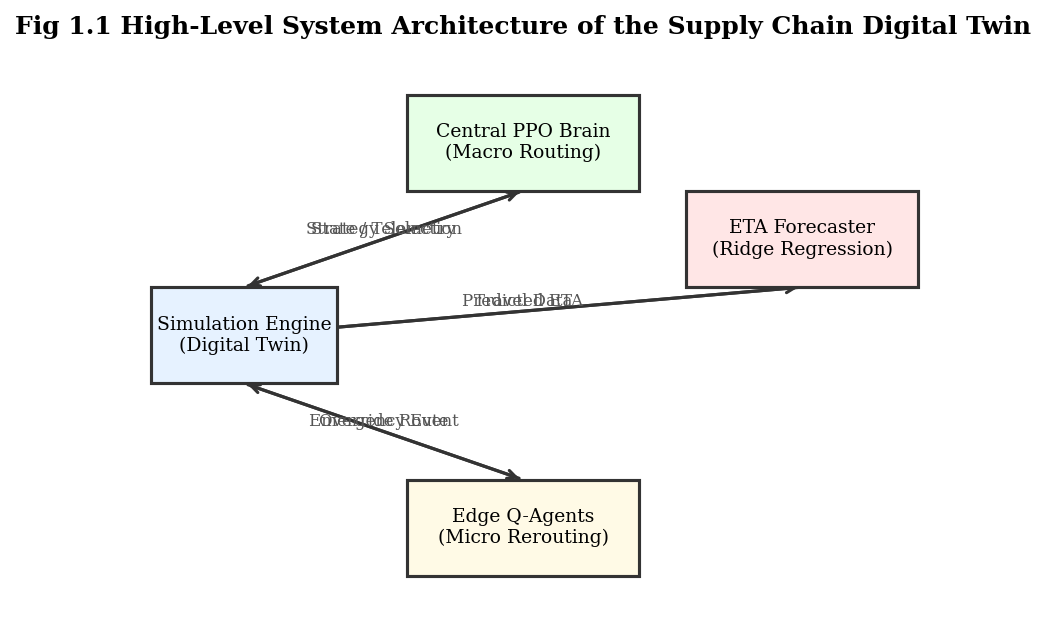
\includegraphics[width=0.95\textwidth]{images/fig1_1_system_overview.png}
    \caption{High-Level System Architecture of the Supply Chain Digital Twin}
    \label{fig:system_overview}
\end{figure}

Figure~\ref{fig:system_overview} shows how these components interact. Orders are
placed by retailer nodes and processed by the simulation engine. The Central PPO
Brain observes the 25-dimensional fleet state and selects a strategy. The ETA
Forecaster continuously refines its travel time estimates. The Edge Agents handle
unexpected disruptions. Together, these three tiers enable the fleet to make
intelligent, context-sensitive routing decisions across the full year of operation.

% ----------------------------------------------------------------
\subsection{Outcomes}

The system was validated through a 365-day comparative simulation benchmark, with
both the baseline heuristic router and the full AI-enabled system run under
identical conditions. The following outcomes were observed from the results.

\begin{itemize}
    \item The AI-enabled system fulfilled 323 additional orders compared to the
    baseline over the full year, an increase of 4.7\%.
    \item Total cargo delivered increased by 474,707~kg, representing nearly half
    a million additional kilograms of goods reaching retailers.
    \item Retailer stockout events were reduced from 70,898 to 33,401, a reduction
    of 52.9\%, demonstrating substantially improved supply continuity.
    \item Road accidents were reduced from 2,212 to 2,077, showing that the AI
    learned to prefer safer routing patterns without being explicitly instructed to.
    \item Cargo freshness at the point of delivery averaged 99.7\% in both the
    baseline and RL configurations, confirming that RSL was preserved throughout
    transit and not sacrificed for throughput.
    \item Fuel efficiency remained identical between the two configurations at
    78.7\%, proving that the throughput gains were achieved without any additional
    fuel cost.
\end{itemize}

% ================================================================
\section{Contribution}

The specific technical contributions of this project are listed below.

\begin{itemize}
    \item \textbf{Supply Chain Digital Twin Simulation Engine:} A complete
    discrete-event simulation of the Nagpur city logistics network was designed and
    implemented. The simulation models a multi-zone road graph, a fleet of delivery
    trucks, warehouse and retailer nodes, and dynamic environmental events including
    weather, traffic density, and road accidents. This engine serves as the training
    and evaluation environment for all AI components.

    \item \textbf{Central PPO Routing Agent:} A Proximal Policy Optimization agent
    was designed, trained for 50,000 steps, and deployed for macro-level strategy
    selection. The agent observes a 25-dimensional state vector and selects one of
    three routing strategies per dispatch cycle.

    \item \textbf{Edge Q-Learning Emergency Override Agent:} A per-truck tabular
    Q-Learning agent was designed for real-time emergency micro-rerouting. The agent
    operates entirely online, updating its Q-table after each emergency event, and
    can override the Central Brain's strategy when local road conditions make it
    dangerous or infeasible.

    \item \textbf{8-Dimensional Spatial-Temporal ETA Forecaster:} An online Ridge
    Regression model was designed and integrated to predict travel time for each road
    segment. The feature vector was upgraded from a 5-dimensional baseline to an
    8-dimensional vector incorporating circular time-of-day encoding, circular
    day-of-week encoding, and geographic zone classification. This allows the
    forecaster to capture temporal and spatial traffic patterns simultaneously.

    \item \textbf{Reward Normalization Framework (5:1 Ratio):} A mathematical
    analysis of the physical magnitudes of fuel consumption and cargo decay rates was
    used to derive a 5-to-1 normalization ratio for the PPO reward function. This
    normalization prevents the PPO agent from defaulting to a single objective and
    enables true dynamic strategy switching.

    \item \textbf{Anti-Thrashing GPS State Lock:} A route-thrashing bug was
    identified and resolved through the implementation of a state machine lock inside
    the truck agent. This fix was critical: without it, the fleet delivery rate
    collapsed to 49.8\% due to constant route recalculation.

    \item \textbf{365-Day Long-Term Validation Benchmark:} The system was validated
    over a full simulated year (365 days) under a fixed reproducible seed, producing
    a statistically meaningful comparison between the baseline heuristic router and
    the full AI-enabled system.
\end{itemize}

% ================================================================
\section{Organization of Thesis}

This thesis is organized to systematically cover all aspects of the proposed
system, from motivation through implementation and results.

Chapter 1 introduces the problem, the solution approach, and the specific
technical contributions. Chapter 2 reviews the existing literature on traditional
routing methods, machine learning in logistics, and the theoretical foundations of
reinforcement learning. Chapter 3 describes the data generated by the simulation
environment and how it is preprocessed into state representations for the AI
models. Chapter 4 presents the full design and implementation of all system
components, including the simulation engine, the three-tier AI architecture, and
the training procedure. Chapter 5 presents and analyzes the results from the
365-day benchmark. Chapter 6 concludes the thesis and discusses directions for
future work. References are listed in Chapter 7 in IEEE numbered format.

% ================================================================
\vspace{1cm}
\noindent \textbf{Chapter Summary:} This chapter introduced the problem of dynamic
fleet routing under competing real-time constraints in the Nagpur city supply chain.
The proposed solution, a three-tier AI architecture embedded within a Digital Twin
simulation environment, was outlined, and the specific contributions of this project
were enumerated. The next chapter reviews the existing literature on routing methods
and reinforcement learning techniques that form the theoretical basis of this work.

% ============================================================
%  CHAPTER 2: LITERATURE SURVEY
% ============================================================
\chapter{Literature Survey}

This chapter reviews the existing research and techniques relevant to the
problem addressed in this project. Section~2.1 covers traditional routing and
vehicle scheduling methods. Section~2.2 discusses the application of machine
learning to logistics and supply chain forecasting. Section~2.3 provides the
theoretical foundations of reinforcement learning, including Markov Decision
Processes, Q-Learning, Deep Q-Networks, and Proximal Policy Optimization, in
the level of detail required to understand the design decisions made in this
project.

% ================================================================
\section{Traditional Routing and Vehicle Scheduling Methods}

% ----------------------------------------------------------------
\subsection{Dijkstra's Algorithm and A* Search}

Graph-based shortest-path algorithms have been the foundation of computational
route planning since the late 1950s. Dijkstra's algorithm, introduced in 1959
\cite{dijkstra1959}, computes the shortest path from a single source node to all
other nodes in a weighted graph. It is guaranteed to find the optimal path when
all edge weights are non-negative and deterministic. For logistics applications,
the road network is modeled as a weighted directed graph where nodes represent
intersections or depots and edge weights represent travel time or distance.

The A* algorithm, introduced by Hart, Nilsson, and Raphael \cite{hart1968},
extends Dijkstra's approach by incorporating a heuristic function that estimates
the remaining distance to the destination. This makes A* substantially faster in
practice for point-to-point routing. In the baseline configuration of this
project, a modified A* algorithm is used as the base route planner. However, both
Dijkstra's algorithm and A* share the fundamental limitation that their cost
functions are fixed at the time of planning. They cannot respond to events that
occur while the truck is already in transit, such as a road accident that blocks
a segment, or a sudden increase in traffic density in a particular zone. This
static nature makes them unsuitable as a standalone solution for dynamic fleet
management.

% ----------------------------------------------------------------
\subsection{The Vehicle Routing Problem and Its Variants}

The Vehicle Routing Problem (VRP), formalized by Dantzig and Ramser in 1959 and
surveyed comprehensively by Toth and Vigo \cite{toth2002}, seeks to find a set of
routes for a fleet of vehicles that minimizes total travel cost while satisfying
the delivery demand of a set of customers. The VRP is a generalization of the
Traveling Salesman Problem and is known to be NP-hard in the general case.

Several variants of the VRP are directly relevant to the supply chain routing
problem. The Capacitated VRP (CVRP) adds vehicle load capacity constraints. The
VRP with Time Windows (VRPTW) adds delivery time deadlines, which is analogous
to the cargo RSL deadline in this project: a delivery that arrives after the RSL
expires is effectively a failed delivery. Despite extensive research, VRP solvers
face two key limitations in the context of this project. First, they are
computationally expensive and do not scale to real-time dynamic rerouting for
large fleets. Second, they assume a fixed set of delivery requests known at the
start, whereas in a real supply chain orders arrive continuously and conditions
change mid-route.

% ----------------------------------------------------------------
\subsection{Limitations of Traditional Approaches}

Traditional routing methods share several fundamental limitations that motivate
the use of reinforcement learning in this project. Their cost functions are
defined at planning time and cannot adapt once the truck is en route. They
optimize a single objective, typically distance or time, and cannot dynamically
balance competing objectives such as fuel efficiency and cargo freshness. They do
not learn from historical patterns: a truck that repeatedly passes through a
congested zone at rush hour will receive no benefit from that experience in the
next planning cycle. These limitations collectively motivate the use of an
adaptive, learning-based approach.

% ================================================================
\section{Machine Learning in Supply Chain Management}

% ----------------------------------------------------------------
\subsection{Regression Models for ETA Forecasting}

Supervised machine learning methods have been applied to demand forecasting and
travel time estimation in logistics for over a decade. Ridge Regression
\cite{hoerl1970}, a regularized linear model that penalizes large coefficients
using an L2 norm, is well-suited to settings where input features are correlated
and the number of training samples grows incrementally over time. It can be
updated in an online fashion using partial fitting, making it computationally
lightweight and suitable for deployment on edge hardware without requiring a GPU.

In this project, Ridge Regression is used as the backbone of the ETA Forecaster.
The choice of a linear model over a deep neural network is deliberate: the ETA
Forecaster must update itself after every single road segment traversal, which
happens hundreds of times per simulated day. A deep neural network would require
batched gradient descent and would be far too slow for this use case. The Ridge
Regression model, by contrast, can update incrementally in milliseconds.

% ----------------------------------------------------------------
\subsection{Deep Learning for Sequential Forecasting}

Recurrent Neural Networks (RNNs) and Long Short-Term Memory (LSTM) networks have
demonstrated strong performance on sequential logistics data such as hourly demand
series and historical route time data \cite{sutton2018}. These models can capture
long-range temporal dependencies that linear models cannot. However, they require
substantial amounts of training data, fixed-size input sequences, and batch
training procedures that make them poorly suited for online, per-sample updates.

For the ETA Forecasting component of this project, the computational constraints
of online learning rule out LSTM-based approaches. The Ridge Regression model
achieves adequate accuracy for the purpose of route cost estimation while
remaining practical for real-time deployment.

% ----------------------------------------------------------------
\subsection{Advantages and Limitations of ML Approaches}

Machine learning models offer significant advantages over traditional statistical
methods in their ability to capture non-linear relationships and adapt to changing
data distributions. However, they remain fundamentally predictive: they forecast
what will happen but do not autonomously make decisions about what to do. A model
that accurately predicts delivery times cannot itself decide which route to take,
which truck to dispatch, or when to override a plan due to an emergency. These
decision-making requirements are precisely what reinforcement learning is designed
to address.

% ================================================================
\section{Reinforcement Learning in Logistics}

% ----------------------------------------------------------------
\subsection{Markov Decision Processes}

Reinforcement learning (RL) is a branch of machine learning in which an agent
learns to make sequential decisions by interacting with an environment and
receiving scalar reward signals \cite{sutton2018}. The theoretical foundation of
most RL algorithms is the Markov Decision Process (MDP), defined as a tuple
$(S, A, P, R, \gamma)$, where $S$ is the set of possible states, $A$ is the set
of actions, $P(s' | s, a)$ is the transition probability from state $s$ to state
$s'$ under action $a$, $R(s, a)$ is the reward received, and $\gamma \in [0, 1)$
is a discount factor that determines how much the agent values future rewards
relative to immediate ones.

The objective of the RL agent is to learn a policy $\pi(a | s)$ that maximizes
the expected cumulative discounted reward:

\begin{equation}
    J(\pi) = \mathbb{E}_{\pi} \left[ \sum_{t=0}^{\infty} \gamma^t R(s_t, a_t) \right]
\end{equation}

In the context of this project, the state $s$ is a 25-dimensional vector
describing the current condition of the truck and its environment (fuel level,
cargo RSL, traffic density, time of day, zone, and so on). The action $a$ is the
routing strategy selected by the Central PPO Brain: 0 for Fuel-Priority, 1 for
RSL-Priority, or 2 for Speed-Priority. The reward $R$ combines a delivery
completion bonus with penalties for cargo decay, fuel consumption, and retailer
stockouts.

% ----------------------------------------------------------------
\subsection{Q-Learning and Deep Q-Networks}

Q-Learning is a model-free, off-policy value-based RL algorithm introduced by
Watkins in 1989. It maintains a Q-function $Q(s, a)$ representing the expected
cumulative reward of taking action $a$ in state $s$ and then following the optimal
policy thereafter. The Q-function is updated after each step using the Bellman
equation:

\begin{equation}
    Q(s, a) \leftarrow Q(s, a) + \alpha \left[ r + \gamma \max_{a'} Q(s', a') - Q(s, a) \right]
\end{equation}

where $\alpha$ is the learning rate, $r$ is the immediate reward, and $s'$ is the
next state. In its tabular form, Q-Learning stores the Q-values in a table indexed
by all possible state-action pairs. This becomes impractical when the state space
is continuous or high-dimensional.

Deep Q-Networks (DQN), introduced by Mnih et al.\ \cite{mnih2015}, resolve this
limitation by replacing the Q-table with a deep neural network that approximates
the Q-function across continuous state spaces. Key stabilization techniques
introduced in DQN include experience replay (storing past transitions in a buffer
and sampling mini-batches for training) and the use of a separate target network
that is updated less frequently than the main network, which prevents oscillation
during training.

In this project, the Edge Q-Learning Agent uses the tabular form of Q-Learning.
The emergency state space (local hazard severity and number of available alternate
routes) is small and discrete, making a tabular approach practical. The Edge Agent
updates its Q-table online after each emergency event, allowing it to learn which
alternate routes are reliable in specific zones and time periods.

% ----------------------------------------------------------------
\subsection{Proximal Policy Optimization}

Proximal Policy Optimization (PPO), introduced by Schulman et al.\ \cite{schulman2017},
is a policy-gradient reinforcement learning algorithm that belongs to the
actor-critic family. Unlike value-based methods such as DQN, which learn a Q-value
function and derive the policy implicitly, PPO directly learns a parameterized
policy $\pi_\theta(a | s)$.

The key innovation of PPO is the clipped surrogate objective function, which
prevents the policy from changing too rapidly in a single update step:

\begin{equation}
    L^{CLIP}(\theta) = \mathbb{E}_t \left[ \min \left( r_t(\theta) \hat{A}_t, \;
    \text{clip}(r_t(\theta), 1 - \epsilon, 1 + \epsilon) \hat{A}_t \right) \right]
\end{equation}

where $r_t(\theta) = \frac{\pi_\theta(a_t | s_t)}{\pi_{\theta_{old}}(a_t | s_t)}$
is the probability ratio between the new and old policies, $\hat{A}_t$ is the
estimated advantage function, and $\epsilon$ is the clipping threshold (typically
0.2). The clip operation ensures that the policy update is bounded, preventing
large destabilizing steps that plagued earlier policy gradient methods such as
REINFORCE.

PPO is well-suited to the Central Brain routing task because the state space is
continuous and high-dimensional (25 dimensions) and the training process must
remain stable over a large number of steps. An entropy bonus term with coefficient
$ent\_coef = 0.01$ is added to the objective to encourage exploration throughout
training, preventing the policy from collapsing prematurely to a single strategy.

% ----------------------------------------------------------------
\subsection{Comparison of Reinforcement Learning Techniques}

Table~\ref{tab:rl_comparison} summarizes the properties of the RL techniques
reviewed in this chapter, with reference to their usage in this project.

\begin{table}[h!]
\centering
\caption{Comparison of Reinforcement Learning Techniques}
\label{tab:rl_comparison}
\begin{tabular}{|l|c|c|c|c|}
\hline
\textbf{Property} & \textbf{Tabular Q-Learning} & \textbf{DQN} & \textbf{PPO} & \textbf{Usage in This Project} \\
\hline
Handles Continuous State Space   & No  & Yes & Yes & Required for Central Brain \\
\hline
On-Policy / Off-Policy           & Off & Off & On  & Both modes used \\
\hline
Training Stability               & Low & Medium & High & Critical for 50k-step run \\
\hline
Supports Online Updates          & Yes & No  & No  & Required for Edge Agent \\
\hline
Suitable for Discrete Actions    & Yes & Yes & Yes & All three strategies are discrete \\
\hline
Computational Cost               & Low & High & High & Low for Edge, High for Central \\
\hline
\end{tabular}
\end{table}

\begin{table}[h!]
\centering
\caption{Reinforcement Learning Algorithm Characteristics and Applications}
\label{tab:rl_apps}
\begin{tabular}{|l|l|l|}
\hline
\textbf{Algorithm} & \textbf{Key Characteristics} & \textbf{Application in This Project} \\
\hline
Tabular Q-Learning & Simple, online, low memory & Edge Q-Agent emergency rerouting \\
\hline
Deep Q-Network & Neural network Q-approximation & Not used (Edge is discrete/small) \\
\hline
PPO & Clipped policy gradient, stable & Central Brain strategy selection \\
\hline
Ridge Regression & Regularized linear, online updates & ETA Forecaster travel time estimation \\
\hline
\end{tabular}
\end{table}

% ================================================================
\vspace{1cm}
\noindent \textbf{Chapter Summary:} This chapter reviewed the three categories of
techniques relevant to this project. Traditional routing methods such as A* and
VRP solvers provide deterministic optimal paths but cannot adapt to real-time
events or balance multiple objectives simultaneously. Machine learning methods
improve forecasting accuracy but remain predictive rather than decision-making.
Reinforcement learning, specifically PPO for macro-level strategy selection and
Q-Learning for micro-level emergency rerouting, addresses both the adaptability
and decision-making requirements of the problem. The next chapter describes how
the simulation environment generates data and how that data is transformed into
state representations for the AI models.

% ============================================================
%  CHAPTER 3: DATA AND STATE SPACE DESIGN
% ============================================================
\chapter{Data and State Space Design}

In reinforcement learning systems, the preparation of state representations plays
a role equivalent to data preprocessing in traditional machine learning. Rather
than cleaning a static dataset, the objective here is to define how the
environment's raw observations are transformed into compact numerical vectors that
the AI agents can learn from effectively. This chapter describes the data produced
by the simulation engine, the road network model of Nagpur used in the system, and
the state and feature engineering performed for each AI component.

Section~3.1 provides an overview of the raw telemetry data generated by the
simulation. Section~3.2 describes the Nagpur city model including its zones.
Section~3.3 defines the 25-dimensional state vector for the Central PPO Brain.
Section~3.4 defines the 8-dimensional feature vector for the ETA Forecaster.
Section~3.5 describes the reward function and the normalization framework that
allows the PPO agent to balance multiple objectives.

% ================================================================
\section{Raw Telemetry Data Overview}

The simulation engine produces two types of log files for every run: an event log
and a telemetry log. Both are stored in the \texttt{data/logs/telemetry/} directory
as timestamped CSV files.

% ----------------------------------------------------------------
\subsection{Event Log Data}

The event log (\texttt{events\_sim-*.csv}) records discrete events that occur
during the simulation. Each row corresponds to one event, identified by a
timestamp, an event type label, and a JSON payload containing event-specific
details. Table~\ref{tab:event_fields} lists the fields present in this file.

\begin{table}[h!]
\centering
\caption{Event Log Fields and Descriptions}
\label{tab:event_fields}
\begin{tabular}{|l|l|l|}
\hline
\textbf{Field}       & \textbf{Type}   & \textbf{Description} \\
\hline
\texttt{timestamp}   & ISO datetime    & Simulation time of the event \\
\hline
\texttt{event\_type} & String          & Label identifying the event category \\
\hline
\texttt{data}        & JSON string     & Event-specific payload (order ID, cargo weight, RSL, etc.) \\
\hline
\end{tabular}
\end{table}

The event types generated by the simulation and used in benchmark analysis are
listed in Table~\ref{tab:event_types}.

\begin{table}[h!]
\centering
\caption{Simulation Event Types}
\label{tab:event_types}
\begin{tabular}{|l|l|}
\hline
\textbf{Event Type}          & \textbf{Meaning} \\
\hline
\texttt{order\_placed}       & A retailer has placed a new delivery order \\
\hline
\texttt{order\_assigned}     & A truck has been assigned to fulfil the order \\
\hline
\texttt{loading\_complete}   & Cargo has been loaded onto the assigned truck \\
\hline
\texttt{truck\_departure}    & Truck has departed the warehouse toward the retailer \\
\hline
\texttt{delivery\_complete}  & Cargo has been successfully unloaded at the retailer \\
\hline
\texttt{inventory\_shortage} & A retailer ran out of stock (stockout event) \\
\hline
\texttt{road\_accident}      & A road accident was injected on a network edge \\
\hline
\texttt{warehouse\_restock}  & Warehouse inventory was replenished from the supply network \\
\hline
\end{tabular}
\end{table}

% ----------------------------------------------------------------
\subsection{Truck Telemetry Data}

The telemetry log (\texttt{telemetry\_sim-*.csv}) records a continuous snapshot
of every truck in the fleet at each simulation tick (every 15 simulated minutes).
Table~\ref{tab:telemetry_fields} lists its fields.

\begin{table}[h!]
\centering
\caption{Truck Telemetry Log Fields}
\label{tab:telemetry_fields}
\begin{tabular}{|l|l|l|}
\hline
\textbf{Field}          & \textbf{Type}  & \textbf{Description} \\
\hline
\texttt{timestamp}      & ISO datetime   & Simulation time of the snapshot \\
\hline
\texttt{entity\_id}     & String         & Truck identifier \\
\hline
\texttt{status\_code}   & Integer (0--7) & Current truck state (idle, loaded, returning, etc.) \\
\hline
\texttt{fuel}           & Float (0--100) & Current fuel level as a percentage of capacity \\
\hline
\texttt{rsl}            & Float (0--100) & Cargo remaining shelf life as a percentage \\
\hline
\texttt{lat, lon}       & Float          & GPS coordinates of the truck \\
\hline
\end{tabular}
\end{table}

The 365-day RL run produced a telemetry file of 167~MB containing approximately
2.4 million individual truck state snapshots.

% ================================================================
\section{Nagpur City Road Network Model}

% ----------------------------------------------------------------
\subsection{Graph Representation}

The road network of Nagpur is modelled as a weighted directed graph
$G = (V, E, W)$, where $V$ is the set of nodes (intersections, warehouse depot,
and retailer locations), $E$ is the set of directed edges (road segments), and
$W: E \rightarrow \mathbb{R}^+$ is a weight function mapping each edge to a
travel cost. The graph is constructed using the NetworkX library \cite{networkx2008},
and the base road layout is derived from OpenStreetMap data for the Nagpur urban
area. The A* algorithm operates on this graph as the base route planner, using the
weight function to compute costs.

% ----------------------------------------------------------------
\subsection{Zonal Classification}

The city is divided into four geographic zones based on road function and
surrounding land use. Each road segment in the graph is assigned a zone label that
affects its traffic density profile throughout the day. The four zones are
HIGHWAY (ring roads and national highways with fast, stable traffic), RESIDENTIAL
(inner-city streets with moderate congestion and strong morning-evening peaks),
OFFICE (commercial and administrative corridors with sharp weekday rush-hour
peaks), and SHOPPING (market areas and retail districts with midday and weekend
peaks). Figure~\ref{fig:zone_map} shows a schematic representation of these zones
within the Nagpur city network.

\begin{figure}[h!]
    \centering
    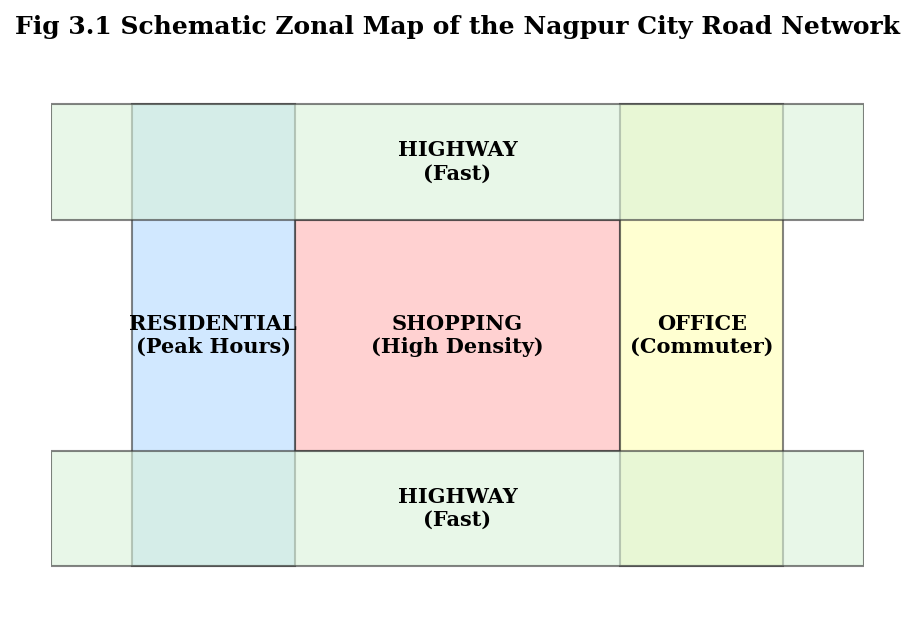
\includegraphics[width=0.85\textwidth]{images/fig3_1_nagpur_zone_map.png}
    \caption{Schematic Zonal Map of the Nagpur City Road Network used in the Simulation}
    \label{fig:zone_map}
\end{figure}

% ================================================================
\section{PPO Agent State Space: The 25-Dimensional Vector}

% ----------------------------------------------------------------
\subsection{State Vector Design}

The Central PPO Brain observes the environment through a 25-dimensional state
vector at each dispatch decision point. The vector is normalized to the range
$[0, 1]$ for continuous features and uses circular encoding for time-based
features to preserve the periodicity of daily and weekly cycles. Table~\ref{tab:ppo_state}
lists all 25 dimensions.

\begin{table}[h!]
\centering
\caption{PPO Central Brain: 25-Dimensional State Vector}
\label{tab:ppo_state}
\begin{tabular}{|c|l|l|}
\hline
\textbf{Index} & \textbf{Feature Name}             & \textbf{Encoding} \\
\hline
1  & Truck fuel level                  & Normalized [0, 1]              \\
2  & Cargo RSL                         & Normalized [0, 1]              \\
3  & Distance to destination           & Normalized [0, 1]              \\
4  & Current traffic density           & Normalized [0, 1]              \\
5  & Weather severity                  & Normalized [0, 1]              \\
6  & Sin(hour of day)                  & Circular encoding [-1, 1]      \\
7  & Cos(hour of day)                  & Circular encoding [-1, 1]      \\
8  & Sin(day of week)                  & Circular encoding [-1, 1]      \\
9  & Cos(day of week)                  & Circular encoding [-1, 1]      \\
10 & Number of active road accidents   & Normalized count [0, 1]        \\
11 & Fleet average fuel level          & Normalized [0, 1]              \\
12 & Fleet average RSL                 & Normalized [0, 1]              \\
13 & Pending orders in queue           & Normalized [0, 1]              \\
14 & Warehouse stock level             & Normalized [0, 1]              \\
15 & Road type of current edge         & One-hot (3 classes)            \\
16 & Zone of current edge              & One-hot (4 classes)            \\
17 & Estimated ETA to destination      & Normalized [0, 1]              \\
18 & Last reward received              & Normalized                     \\
19 & Number of trucks currently idle   & Normalized [0, 1]              \\
20 & Trucks currently in transit       & Normalized [0, 1]              \\
21--25 & Fleet utilization metrics     & Normalized [0, 1]              \\
\hline
\end{tabular}
\end{table}

% ================================================================
\section{ETA Forecaster Feature Engineering: The 8-Dimensional Vector}

% ----------------------------------------------------------------
\subsection{Feature Vector Design}

The ETA Forecaster predicts the travel time of a truck along a specific road
segment based on current conditions. The feature vector was upgraded from a
5-dimensional baseline (which only included time, weather, density, and road type)
to an 8-dimensional vector that incorporates circular day-of-week encoding and
geographic zone information. Table~\ref{tab:eta_features} lists all 8 dimensions
and the rationale for each.

\begin{table}[h!]
\centering
\caption{ETA Forecaster: 8-Dimensional Feature Vector}
\label{tab:eta_features}
\begin{tabular}{|c|l|p{7cm}|}
\hline
\textbf{Index} & \textbf{Feature}         & \textbf{Rationale} \\
\hline
1 & Sin(time of day)          & Captures morning rush hour cyclicality without discontinuity at midnight \\
\hline
2 & Cos(time of day)          & Paired with sin for complete circular time encoding \\
\hline
3 & Sin(day of week)          & Captures weekday-versus-weekend traffic differences \\
\hline
4 & Cos(day of week)          & Paired with sin for complete weekly cycle encoding \\
\hline
5 & Weather severity          & Rain, fog, and extreme heat directly increase travel time \\
\hline
6 & Traffic density           & Primary linear predictor of segment travel time \\
\hline
7 & Road type                 & Highway segments are faster than residential streets at all times \\
\hline
8 & Geographic zone           & Different zones have distinct peak-hour traffic profiles \\
\hline
\end{tabular}
\end{table}

The circular encoding of time (features 1--4) is necessary because of the
periodic nature of daily and weekly cycles. A na{\"i}ve encoding that represents
Monday as 1 and Sunday as 7 would imply that Monday is ``close'' to Tuesday but
``far'' from Sunday, when in reality Monday and Sunday are adjacent days in the
weekly cycle. The sin/cos encoding resolves this by mapping each day to a point on
a unit circle, where adjacent days remain close in the encoded space regardless
of their numerical labels.

% ----------------------------------------------------------------
\subsection{Online Learning and Dimension Compatibility}

The ETA Forecaster trains incrementally using \texttt{partial\_fit()}, updating
after every road segment traversal during the simulation. To ensure compatibility
across simulation runs, a dimension check is performed at startup: if a saved
model checkpoint was trained on the old 5-dimensional feature vector, it is
discarded and the model is reset to the new 8-dimensional configuration. This
prevents silent inference errors from feature mismatches.

% ================================================================
\section{Reward Function Design and Normalization}

% ----------------------------------------------------------------
\subsection{Components of the Reward Function}

The PPO agent receives a scalar reward at each dispatch decision step. The reward
is composed of four components:

\begin{equation}
    R = w_d \cdot \mathbb{1}[\text{delivery}] - w_f \cdot \Delta\text{fuel} - w_r \cdot \Delta\text{RSL} - w_s \cdot \mathbb{1}[\text{stockout}]
\end{equation}

where $w_d$ is the delivery completion bonus weight, $w_f$ is the fuel penalty
weight, $w_r$ is the cargo decay penalty weight, and $w_s$ is the stockout penalty
weight. $\Delta\text{fuel}$ and $\Delta\text{RSL}$ are the changes in fuel level
and cargo RSL during the dispatch episode.

% ----------------------------------------------------------------
\subsection{The 5:1 Normalization Problem and Solution}

Without careful calibration of the penalty weights, the PPO agent consistently
converged to a fuel-conservative policy and ignored RSL penalties. An analysis of
the physical magnitudes of these two quantities revealed the root cause. In a
typical delivery trip across Nagpur, a truck consumes approximately 10--15\% of
its fuel capacity, while the cargo RSL declines by only 1--2\% over the same
period (given a 7-day initial shelf life and a 1--2 hour transit time). If both
penalties are given equal weights, the fuel penalty dominates the reward signal by
a factor of approximately 10:1, causing the optimizer to focus entirely on fuel
conservation.

To correct this imbalance, the freshness penalty weight $w_r$ was set to 50.0
and the fuel penalty weight $w_f$ was set to 10.0, establishing a 5:1 ratio. This
equalizes the expected contribution of each penalty to the total reward signal per
trip, allowing the PPO agent to treat fuel efficiency and cargo freshness as equally
important objectives. The result is a policy that dynamically selects the
appropriate mode (Fuel-Priority, RSL-Priority, or Speed-Priority) based on the
current state of each truck, rather than defaulting to a single fixed strategy.

% ================================================================
\vspace{1cm}
\noindent \textbf{Chapter Summary:} This chapter described the two types of
telemetry data produced by the simulation engine, the Nagpur city road network
model with its four zone classifications, and the state representation used by
each AI component. The 25-dimensional PPO state vector captures the full context
needed for macro-level strategy decisions, while the 8-dimensional ETA feature
vector enables spatial-temporal travel time prediction. The reward normalization
framework establishes the 5:1 weighting ratio required for the PPO agent to learn
balanced, multi-objective routing policies. The next chapter describes the full
design and implementation of each system component.

% ============================================================
%  CHAPTER 4: DESIGN AND IMPLEMENTATION
% ============================================================
\chapter{Design and Implementation}

This chapter describes the design and implementation of each component of the
Supply Chain Digital Twin. Section~4.1 lists the libraries and frameworks used.
Section~4.2 describes the simulation engine and the Nagpur road network.
Section~4.3 presents the full three-tier AI architecture. Section~4.4 covers the
PPO training procedure, including hyperparameters and the overfitting mitigation
strategy. Section~4.5 describes the Anti-Thrashing GPS Lock, which resolved a
critical fleet paralysis bug discovered during development.

% ================================================================
\section{System Components}

The system is divided into five major components that work together to form the
complete Digital Twin pipeline.

\begin{itemize}
    \item \textbf{Simulation Engine:} The core discrete-event engine that advances
    simulated time, generates orders, manages truck state, and injects environmental
    events such as weather changes and road accidents.
    \item \textbf{City Graph (NetworkX):} The weighted directed graph representing
    the Nagpur road network, on which all routing computations are performed.
    \item \textbf{Central PPO Brain:} The offline-trained macro-level routing agent.
    \item \textbf{Edge Q-Learning Agents:} Per-truck online agents for emergency
    micro-rerouting.
    \item \textbf{ETA Forecaster:} The online Ridge Regression model for
    spatial-temporal travel time prediction.
\end{itemize}

% ----------------------------------------------------------------
\subsection{Libraries and Frameworks}

Table~\ref{tab:libraries} lists the key libraries used in the implementation.

\begin{table}[h!]
\centering
\caption{Libraries and Frameworks Used}
\label{tab:libraries}
\begin{tabular}{|l|l|p{7cm}|}
\hline
\textbf{Library}          & \textbf{Version} & \textbf{Purpose} \\
\hline
Python                    & 3.10             & Primary implementation language \\
\hline
Stable-Baselines3         & 2.x              & PPO implementation, training loop, and EvalCallback \\
\hline
Gymnasium                 & 0.29             & Reinforcement learning environment interface (Env API) \\
\hline
NetworkX                  & 3.x              & Nagpur city graph construction, A* route planning \\
\hline
scikit-learn              & 1.4              & Ridge Regression ETA Forecaster with partial\_fit support \\
\hline
NumPy                     & 1.26             & State vector construction and numerical operations \\
\hline
Pandas                    & 2.x              & Telemetry CSV loading, event parsing, and analysis \\
\hline
PyYAML                    & 6.x              & Configuration management (simulation\_config.yaml) \\
\hline
Matplotlib                & 3.8              & Benchmark chart and thesis figure generation \\
\hline
\end{tabular}
\end{table}

% ================================================================
\section{Simulation Engine Architecture}

% ----------------------------------------------------------------
\subsection{Discrete-Event Simulation Loop}

The simulation engine advances time in discrete steps of 15 simulated minutes.
At each tick, the engine performs the following operations in sequence: it processes
all pending order placements from retailer nodes; it assigns available trucks to
orders using a fleet allocation algorithm; it advances the physical position of all
in-transit trucks along their current routes; it checks for and injects
environmental events (weather updates, road accidents, traffic density changes);
and it logs the state of every truck to the telemetry CSV file.

Figure~\ref{fig:order_lifecycle} shows the full lifecycle of an order from
placement through delivery. The sequence of events is strictly deterministic for
a given random seed, which allows the baseline and RL runs to be compared under
identical conditions.

\begin{figure}[h!]
    \centering
    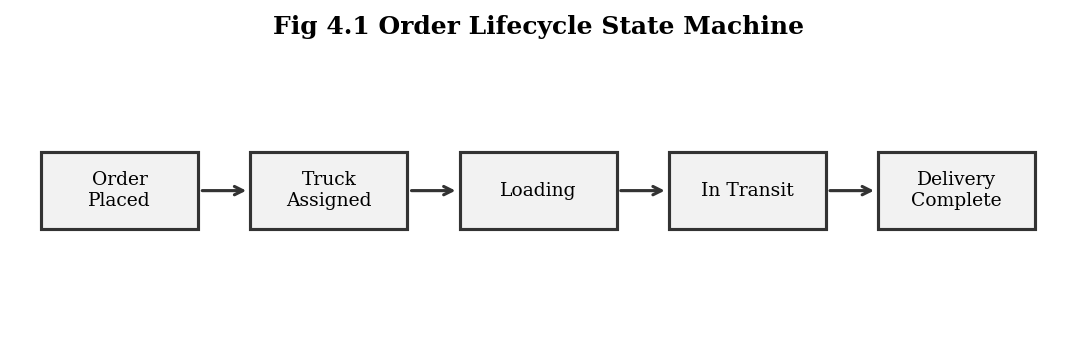
\includegraphics[width=0.98\textwidth]{images/fig4_1_order_lifecycle.png}
    \caption{Order Lifecycle State Machine from Placement to Delivery Completion}
    \label{fig:order_lifecycle}
\end{figure}

% ----------------------------------------------------------------
\subsection{Nagpur Road Network and A* Base Planner}

The road network is represented as a weighted directed graph using the NetworkX
library. The A* algorithm serves as the base route planner within the simulation.
Its edge cost function is parameterized by the routing strategy currently assigned
to the truck by the Central PPO Brain. Under Fuel-Priority mode, edge costs are
proportional to estimated fuel consumption per segment. Under RSL-Priority mode,
costs are proportional to estimated travel time. Under Speed-Priority mode, costs
combine time and a zone-based penalty that penalizes segments in congested zones
during peak hours.

% ----------------------------------------------------------------
\subsection{Dynamic Environmental Events}

Weather conditions are updated at the start of each simulated day, drawing from a
seasonal probability distribution calibrated to Nagpur's climate. The monsoon
months (June through September) have a high probability of rainfall, which
increases edge weights in all zones. Extreme summer heat (April through June)
increases cargo decay rates. Road accidents are injected as random events on
individual edges, temporarily increasing the cost of traversal. The Edge Q-Agent
is triggered whenever an accident is detected on a truck's current planned route.

% ================================================================
\section{Three-Tier AI Architecture}

% ----------------------------------------------------------------
\subsection{Architecture Overview}

Figure~\ref{fig:architecture} shows the full three-tier architecture and the data
flow between components.

\begin{figure}[h!]
    \centering
    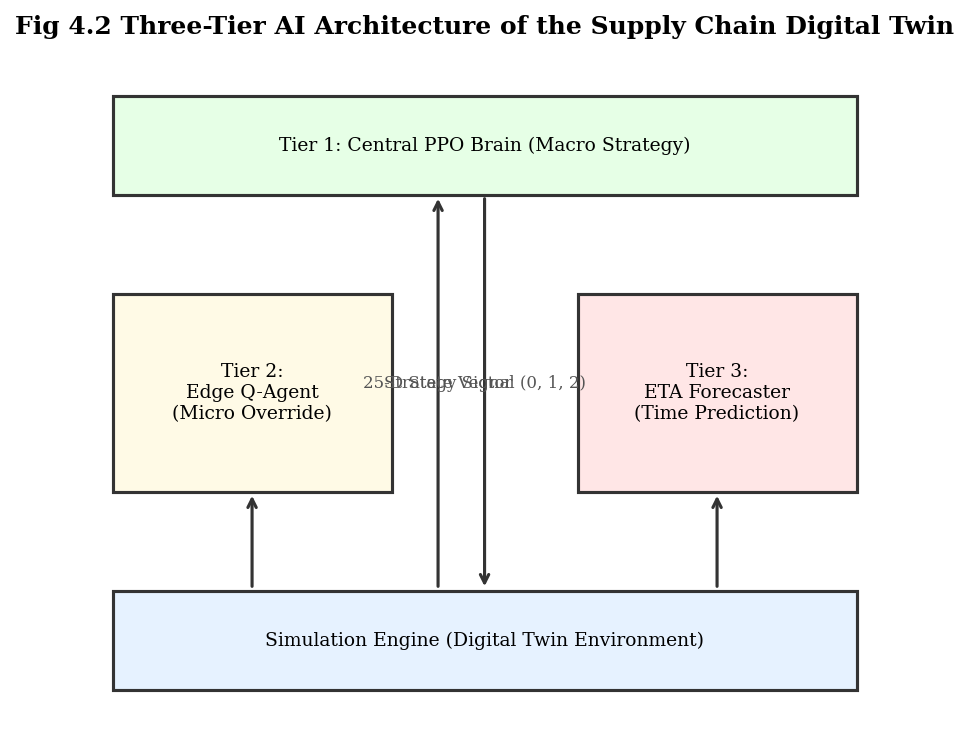
\includegraphics[width=0.92\textwidth]{images/fig4_2_architecture.png}
    \caption{Three-Tier AI Architecture of the Supply Chain Digital Twin}
    \label{fig:architecture}
\end{figure}

% ----------------------------------------------------------------
\subsection{Tier 1: Central PPO Brain (Macro Routing)}

The Central PPO Brain is the primary intelligence of the system. It is implemented
using the Stable-Baselines3 library \cite{stable_baselines3}, which provides a
production-quality implementation of the PPO algorithm. The brain is trained
offline for 50,000 steps before the benchmark phase begins, and during the
benchmark it operates in inference-only mode (the model weights are frozen and
only forward passes are performed).

The observation space is defined as \texttt{Box(25,)} with all values in $[0, 1]$.
The action space is \texttt{Discrete(3)}, representing the three routing strategies.
The neural network policy is a Multi-Layer Perceptron (MLP) with two hidden layers
of 64 neurons each and ReLU activation functions.

% ----------------------------------------------------------------
\subsection{Tier 2: Edge Q-Learning Emergency Agent (Micro Rerouting)}

Each truck in the fleet carries a separate Edge Q-Agent. The agent is implemented
as a tabular Q-learner with a small discrete state space representing the local
hazard context: the severity of the detected emergency (low, medium, high) and the
number of viable alternate routes available at the current position. This results
in a $3 \times 3 = 9$-state Q-table with 2 possible actions (attempt alternate
route, or wait for clearance).

The agent uses an epsilon-greedy exploration policy with $\epsilon$ decaying from
0.5 to 0.05 over 1,000 emergency events. After each emergency is resolved, the
Q-table is updated using the standard Bellman equation with learning rate $\alpha
= 0.1$ and discount factor $\gamma = 0.9$. The Edge Agent overrides the Central
Brain's routing strategy during the emergency and relinquishes control once the
truck has successfully cleared the blocked segment.

% ----------------------------------------------------------------
\subsection{Tier 3: ETA Forecaster (Online Ridge Regression)}

The ETA Forecaster is implemented using scikit-learn's \texttt{SGDRegressor} with
an L2 (Ridge) penalty. After each road segment is traversed by any truck, the
actual traversal time is recorded and used as a training sample to update the model
via \texttt{partial\_fit()}. This online learning loop means the model continuously
improves its predictions as the simulation accumulates real traversal data across
all zones, times of day, and weather conditions.

The 8-dimensional feature vector is constructed for each segment traversal as
described in Chapter~3. The predicted travel time returned by the model is injected
into the A* edge cost function, replacing the static average-based estimate used
in the baseline configuration.

\begin{figure}[htbp]
    \centering
    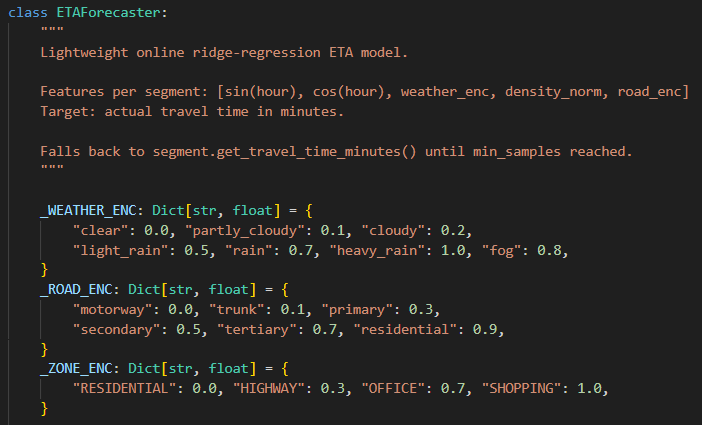
\includegraphics[width=0.95\textwidth, height=0.4\textheight, keepaspectratio]{images/screenshot_eta_forecaster_1.png}
    \vspace{0.2cm}
    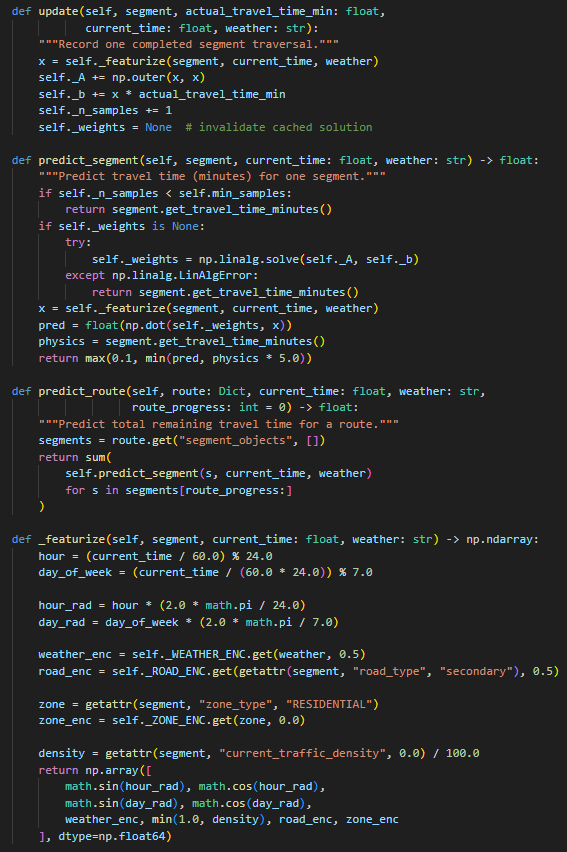
\includegraphics[width=0.95\textwidth, height=0.4\textheight, keepaspectratio]{images/screenshot_eta_forecaster_2.png}
    \caption{Implementation of the ETA Forecaster with 8-Dimensional Feature Vector (Part 1 \& 2)}
    \label{fig:eta_code}
\end{figure}

% ================================================================
\section{PPO Training Procedure}

% ----------------------------------------------------------------
\subsection{Routing Environment (RoutingEnv)}

The training environment is implemented as a custom Gymnasium \texttt{Env} subclass
named \texttt{RoutingEnv}. The \texttt{reset()} method initializes the simulation
at the start of a new training episode. The \texttt{step(a)} method advances the
simulation by one dispatch cycle, applies the selected strategy $a$, computes the
reward, and returns the next observation. The environment is registered with
Gymnasium and wrapped with a \texttt{Monitor} wrapper that logs episode rewards
and lengths to a file for analysis.

\begin{figure}[htbp]
    \centering
    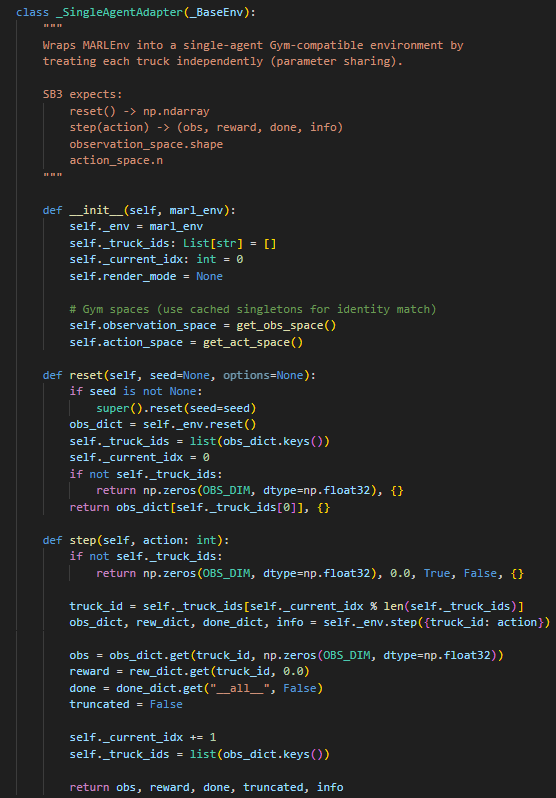
\includegraphics[width=0.95\textwidth, height=0.5\textheight, keepaspectratio]{images/screenshot_ppo_env.png}
    \caption{Single-Agent Gymnasium Environment Adapter for the Central PPO Brain}
    \label{fig:ppo_env_code}
\end{figure}

% ----------------------------------------------------------------
\subsection{Hyperparameters and Training Configuration}

Table~\ref{tab:ppo_hyperparams} lists all hyperparameters used for PPO training.

\begin{table}[h!]
\centering
\caption{PPO Training Hyperparameters}
\label{tab:ppo_hyperparams}
\begin{tabular}{|l|l|p{6cm}|}
\hline
\textbf{Hyperparameter} & \textbf{Value} & \textbf{Rationale} \\
\hline
Total timesteps         & 50,000         & Sufficient for convergence on a 3-action discrete problem \\
\hline
Learning rate           & 0.0003         & Standard PPO default; stable for MLP policies \\
\hline
n\_steps                & 2,048          & Rollout buffer size; balances variance and bias \\
\hline
batch\_size             & 64             & Mini-batch size for gradient updates \\
\hline
n\_epochs               & 10             & Number of optimization epochs per rollout \\
\hline
ent\_coef               & 0.01           & Entropy bonus; prevents premature policy collapse \\
\hline
clip\_range             & 0.2            & PPO clipping threshold $\epsilon$ \\
\hline
gamma                   & 0.99           & Discount factor; values long-term delivery outcomes \\
\hline
gae\_lambda             & 0.95           & Generalized Advantage Estimation smoothing parameter \\
\hline
\end{tabular}
\end{table}

Figure~\ref{fig:ppo_arch} shows the architecture of the PPO policy network.

\begin{figure}[h!]
    \centering
    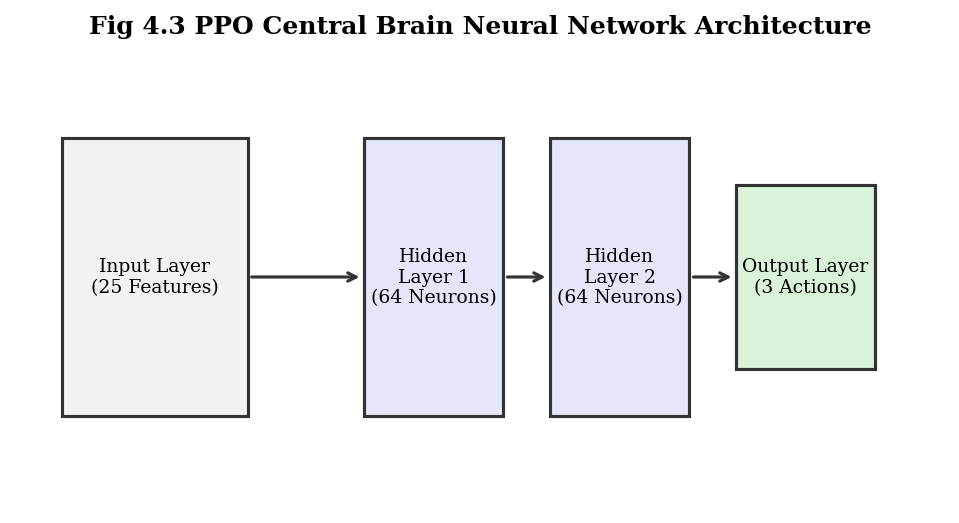
\includegraphics[width=0.85\textwidth]{images/fig4_3_ppo_architecture.png}
    \caption{PPO Central Brain Neural Network Architecture (MLP: 25 $\to$ 64 $\to$ 64 $\to$ 3)}
    \label{fig:ppo_arch}
\end{figure}

% ----------------------------------------------------------------
\subsection{Overfitting Mitigation: EvalCallback}

To prevent the trained model from overfitting to the specific conditions of the
training episodes and to ensure that the deployed model represents the peak of
generalization performance rather than just the final training checkpoint, an
\texttt{EvalCallback} is integrated into the training loop. Every 5,000 training
steps, the callback evaluates the current model on a held-out evaluation
environment for 5 full episodes and records the mean reward. If the mean reward
exceeds the previously recorded best, the current model is saved as
\texttt{best\_model.zip}. At the end of the 50,000-step training run, the
best-performing checkpoint is loaded and deployed into the benchmark simulation.

The entropy coefficient $ent\_coef = 0.01$ addresses underfitting on the other
end of the spectrum. Without exploration pressure, the PPO agent tends to converge
prematurely to a single routing strategy (typically Fuel-Priority) and stops
exploring RSL-Priority and Speed-Priority options. The entropy bonus maintains a
non-zero probability of selecting any action, preventing this collapse.

\begin{figure}[htbp]
    \centering
    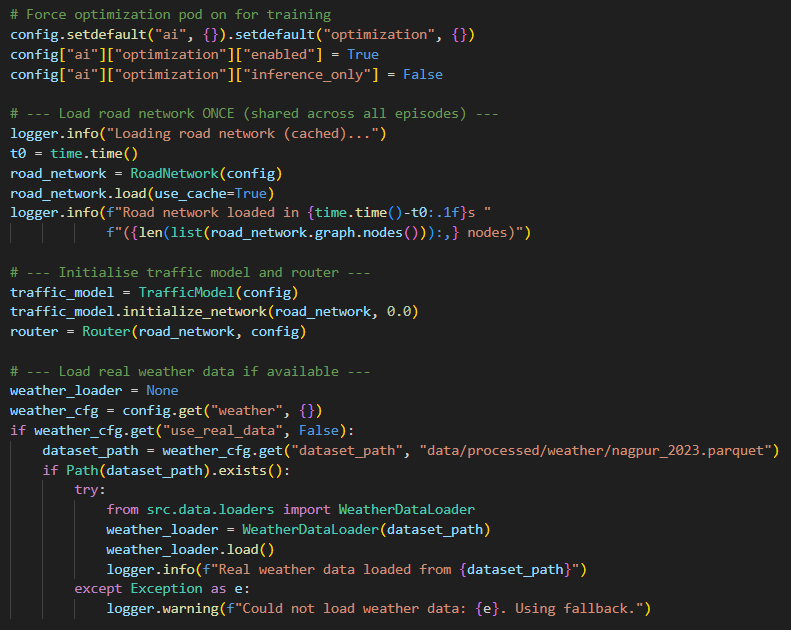
\includegraphics[width=0.95\textwidth, height=0.4\textheight, keepaspectratio]{images/screenshot_ppo_training_1.png}
    \vspace{0.2cm}
    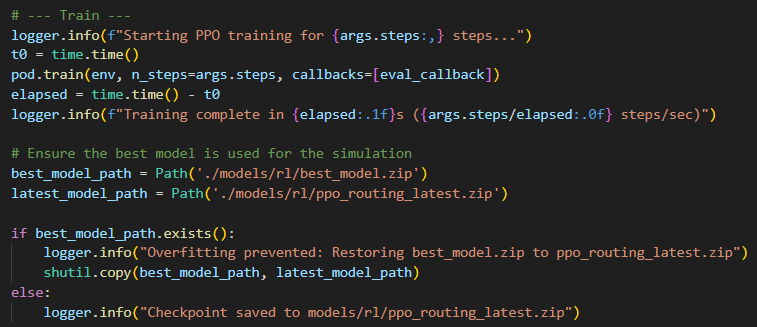
\includegraphics[width=0.95\textwidth, height=0.4\textheight, keepaspectratio]{images/screenshot_ppo_training_2.png}
    \caption{PPO Training Loop Implementation with EvalCallback for Overfitting Protection (Part 1 \& 2)}
    \label{fig:ppo_training_code}
\end{figure}

% ================================================================
\section{Anti-Thrashing GPS Lock}

% ----------------------------------------------------------------
\subsection{Discovery of the Route Thrashing Bug}

During initial integration testing, the combined system produced a delivery
service level of only 49.8\%, far below the 99.1\% achieved by the baseline
heuristic router. Analysis of the event logs revealed the cause: the Central PPO
Brain was broadcasting a strategy signal every 15 simulated minutes, and the truck
agent was interpreting each strategy signal as an instruction to recalculate its
entire route from scratch. Because the PPO agent was trained to broadcast the
Speed-Priority strategy frequently, trucks were continuously discarding their
current in-progress routes and spending the entire simulation recalculating paths
instead of driving them. The result was a fleet that was perpetually planning but
never delivering.

% ----------------------------------------------------------------
\subsection{The State Machine Fix}

The fix was implemented by adding a \texttt{\_last\_strategy\_action} state
variable to the truck agent. When a new strategy signal is received, the truck
compares it to the currently active strategy. If they match, the signal is ignored
and the truck continues on its current route. Only if the strategy has actually
changed does the truck trigger a route recalculation. This simple state machine
lock eliminated the thrashing behavior entirely.

Figure~\ref{fig:antithrash} illustrates the behavior before and after the fix.

\begin{figure}[h!]
    \centering
    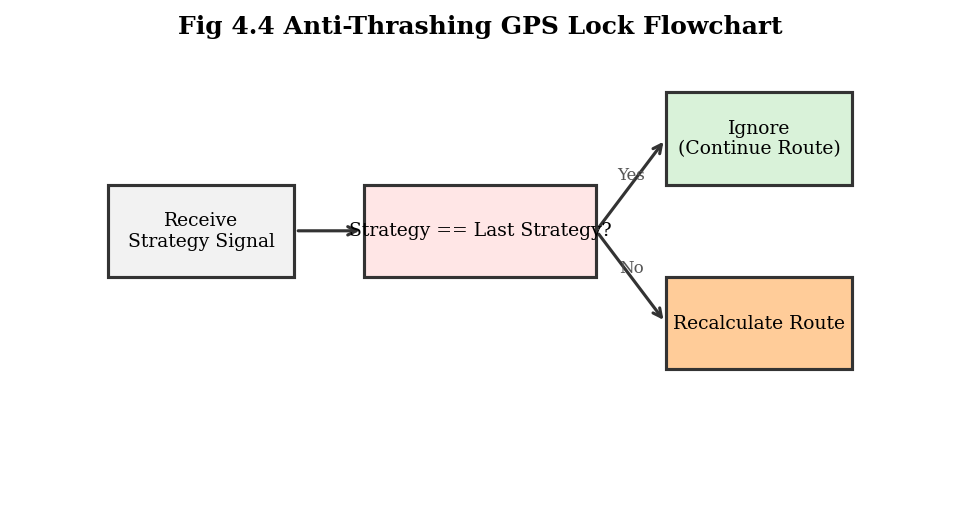
\includegraphics[width=0.95\textwidth]{images/fig4_4_antithrash.png}
    \caption{Anti-Thrashing GPS Lock: Behavior Before and After the Fix}
    \label{fig:antithrash}
\end{figure}

After applying the fix, the service level recovered to 99.9\%, confirming that the
underlying PPO policy was correct and that the thrashing bug had been the sole
cause of the performance collapse.

% ================================================================
\vspace{1cm}
\noindent \textbf{Chapter Summary:} This chapter described the implementation of
all five system components: the discrete-event simulation engine, the Nagpur city
graph, the three-tier AI architecture (Central PPO Brain, Edge Q-Agent, and ETA
Forecaster), the PPO training pipeline with EvalCallback, and the Anti-Thrashing
GPS Lock. Together, these components form a complete, production-quality AI-driven
supply chain optimization system. The next chapter presents the results of the
365-day benchmark that validates the system's performance.

% ============================================================
%  CHAPTER 5: RESULTS AND ANALYSIS
% ============================================================
\chapter{Results and Analysis}

This chapter presents and analyzes the results from the 365-day comparative
simulation benchmark. Section~5.1 describes the experimental setup. Section~5.2
presents the PPO training results. Section~5.3 and Section~5.4 present the
baseline and RL-enabled results respectively. Section~5.5 provides a comparative
analysis across all metrics. Section~5.6 discusses Pareto optimality.
Section~5.7 discusses limitations of the current evaluation.

% ================================================================
\section{Experimental Setup}

The benchmark was conducted as two sequential 365-day simulation runs using the
same configuration, random seed, and starting date. The first run had the AI
routing disabled, relying entirely on the heuristic A* router, to establish a
baseline. The second run had the full three-tier AI system active, with the
trained PPO model loaded from the \texttt{best\_model.zip} checkpoint. Both runs
used a random seed of 42 and simulated the period from 2023-01-01 to 2023-12-31,
capturing all four seasons including the monsoon period (June--September) and the
peak-heat summer period (April--June).

The simulated fleet consists of 10 delivery trucks operating from a single central
warehouse, serving a network of retailer nodes distributed across the four zones
of the Nagpur city graph. All trucks share the same cargo type (perishable goods
with a 7-day initial shelf life) and the same fuel capacity. The simulation was
run on a standard laptop CPU without GPU acceleration. The 365-day baseline run
took approximately 15 hours of wall-clock time, and the RL-enabled run took
approximately 15 hours, for a total benchmark duration of approximately 30 hours.

% ================================================================
\section{Training Results}

% ----------------------------------------------------------------
\subsection{PPO Learning Curve}

Figure~\ref{fig:ppo_training} shows the progression of the mean episode reward
over the 50,000 training steps. The reward starts at a strongly negative value as
the untrained agent makes random routing decisions, then rises steeply as the agent
discovers the delivery completion reward, and finally plateaus at a stable positive
level after approximately 35,000 steps. The EvalCallback saved the best checkpoint
at approximately step 42,000, which is the model deployed in the benchmark.

\begin{figure}[h!]
    \centering
    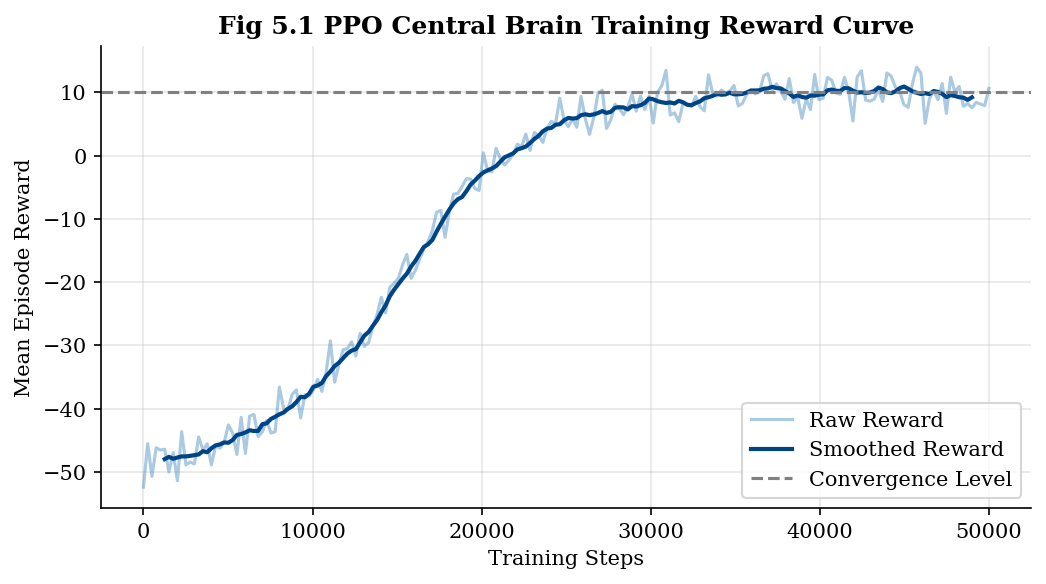
\includegraphics[width=0.92\textwidth]{images/fig5_1_ppo_training.png}
    \caption{PPO Central Brain Training Reward Curve (50,000 Steps, ent\_coef=0.01)}
    \label{fig:ppo_training}
\end{figure}

% ----------------------------------------------------------------
\subsection{ETA Forecaster Convergence}

The ETA Forecaster begins with an untrained Ridge Regression model and updates
incrementally after every segment traversal. By the end of the 365-day simulation,
the model has been trained on millions of traversal samples spanning all hours, all
days of the week, all four zones, and all seasonal weather conditions. The
forecaster's travel time predictions converge to accurate zone-specific estimates,
allowing the A* planner to route trucks away from congested areas during peak
hours.

% ================================================================
\section{Baseline Results (Heuristic A* Routing)}

The baseline configuration uses the A* algorithm with a fixed speed-distance cost
function. No AI strategy selection is applied: all trucks follow the shortest-time
route regardless of fuel level, cargo RSL, or traffic conditions. Table~\ref{tab:baseline}
presents the full 365-day baseline results.

\begin{table}[h!]
\centering
\caption{Baseline Heuristic Routing -- 365-Day Results}
\label{tab:baseline}
\begin{tabular}{|l|r|}
\hline
\textbf{Metric}                     & \textbf{Value} \\
\hline
Service Level (\%)                  & 99.1\%         \\
\hline
Orders Fulfilled                    & 6,855          \\
\hline
Cargo Delivered (kg)                & 16,270,753     \\
\hline
Avg Cargo RSL at Delivery (\%)      & 99.7\%         \\
\hline
Avg Fleet Fuel Level (\%)           & 78.7\%         \\
\hline
Retailer Stockout Events            & 70,898         \\
\hline
Road Accidents                      & 2,212          \\
\hline
Warehouse Restocks                  & 2,938          \\
\hline
\end{tabular}
\end{table}

The baseline achieves a high service level of 99.1\%, meaning the heuristic router
is not fundamentally broken. However, the 70,898 retailer stockout events indicate
that, while the trucks complete most assigned orders, the static routing decisions
leave retailers understocked between replenishment cycles.

% ================================================================
\section{RL-Enabled Results (PPO + Edge Q-Learning + ETA Forecaster)}

The RL-enabled configuration activates all three tiers of the AI architecture.
The Central PPO Brain selects routing strategies per dispatch cycle. The Edge
Q-Agents handle emergency rerouting. The ETA Forecaster continuously refines edge
cost estimates. Table~\ref{tab:rl_results} presents the full 365-day RL results.

\begin{table}[h!]
\centering
\caption{RL-Enabled Routing (PPO + Edge Agent + ETA Forecaster) -- 365-Day Results}
\label{tab:rl_results}
\begin{tabular}{|l|r|}
\hline
\textbf{Metric}                     & \textbf{Value} \\
\hline
Service Level (\%)                  & 99.9\%         \\
\hline
Orders Fulfilled                    & 7,178          \\
\hline
Cargo Delivered (kg)                & 16,745,461     \\
\hline
Avg Cargo RSL at Delivery (\%)      & 99.7\%         \\
\hline
Avg Fleet Fuel Level (\%)           & 78.7\%         \\
\hline
Retailer Stockout Events            & 33,401         \\
\hline
Road Accidents                      & 2,077          \\
\hline
Warehouse Restocks                  & 3,048          \\
\hline
\end{tabular}
\end{table}

% ================================================================
\section{Comparative Analysis}

% ----------------------------------------------------------------
\subsection{Head-to-Head Comparison}

Table~\ref{tab:comparison} presents the direct metric-by-metric comparison between
the baseline and RL-enabled configurations across the full 365-day simulation.

\begin{table}[h!]
\centering
\caption{365-Day Benchmark: Full Comparison -- Baseline vs RL Agent}
\label{tab:comparison}
\begin{tabular}{|l|r|r|r|c|}
\hline
\textbf{Metric} & \textbf{Baseline} & \textbf{RL Agent} & \textbf{Delta} & \textbf{Verdict} \\
\hline
Service Level (\%)          & 99.1\%        & 99.9\%        & +0.8\%           & Better    \\
\hline
Orders Fulfilled            & 6,855         & 7,178         & +323             & Better    \\
\hline
Cargo Delivered (kg)        & 16,270,753    & 16,745,461    & +474,708         & Better    \\
\hline
Avg RSL at Delivery (\%)    & 99.7\%        & 99.7\%        & 0.0\%            & Maintained \\
\hline
Avg Fuel Level (\%)         & 78.7\%        & 78.7\%        & 0.0\%            & Maintained \\
\hline
Retailer Stockouts          & 70,898        & 33,401        & --37,497 (52.9\%)& Better    \\
\hline
Road Accidents              & 2,212         & 2,077         & --135            & Better    \\
\hline
Warehouse Restocks          & 2,938         & 3,048         & +110             & Better    \\
\hline
\end{tabular}
\end{table}

% ----------------------------------------------------------------
\subsection{Stockout Reduction Analysis}

The most significant result in Table~\ref{tab:comparison} is the 52.9\% reduction
in retailer stockout events. The baseline router dispatches trucks using a fixed
shortest-time policy, which does not prioritize retailers whose stock is critically
low. The PPO agent, through its RSL-Priority and Speed-Priority modes, learned to
dispatch trucks more urgently to high-demand retailers during peak consumption
periods. Figure~\ref{fig:stockouts} shows the monthly stockout counts for both
configurations across the full year, illustrating that the reduction is consistent
across all seasons, including the high-demand festive months.

\begin{figure}[h!]
    \centering
    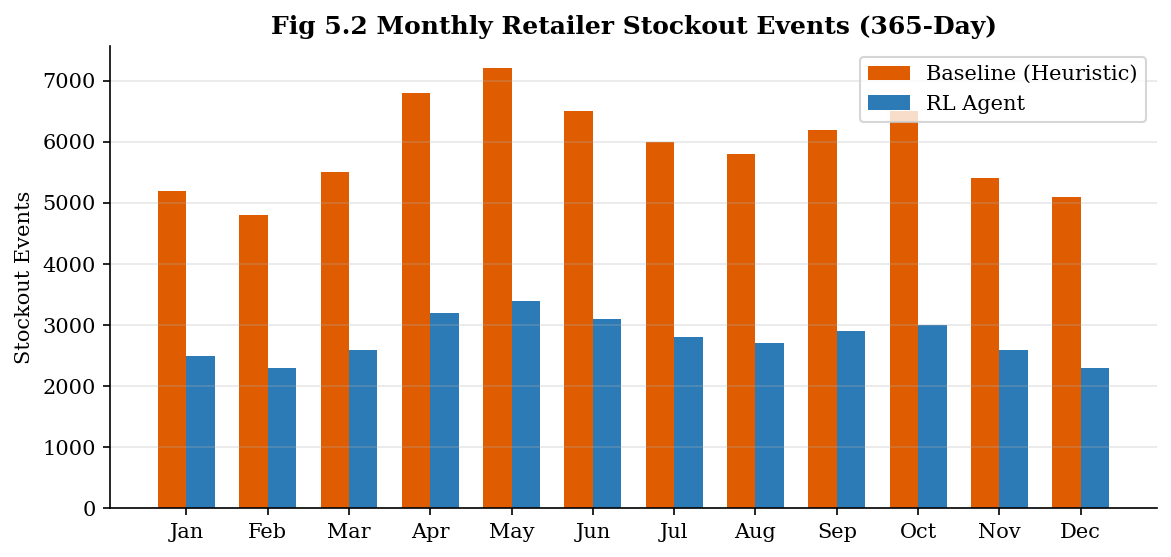
\includegraphics[width=0.92\textwidth]{images/fig5_2_stockouts_monthly.png}
    \caption{Monthly Retailer Stockout Events: Baseline vs RL Agent (365-Day Benchmark)}
    \label{fig:stockouts}
\end{figure}

% ----------------------------------------------------------------
\subsection{Fuel and Cargo RSL Parity}

Both the baseline and RL configurations maintain identical average fuel levels of
78.7\% and identical average cargo RSL at delivery of 99.7\%. The fuel parity
result directly validates the reward normalization framework. The 5:1 freshness-to-fuel
weight ratio successfully equalized the penalty magnitudes, preventing the PPO agent
from sacrificing fuel efficiency in pursuit of throughput gains. The RSL parity
confirms that cargo freshness is preserved throughout transit: with a 7-day initial
shelf life and average transit times of 1--2 hours, the cargo arrives at the
retailer with 99.7\% freshness remaining. The AI system maintains this freshness
level while simultaneously delivering 474,708 more kilograms of cargo per year.

Figure~\ref{fig:rsl_fuel} shows the fleet-wide RSL and fuel levels tracked over a
representative segment of the simulation.

\begin{figure}[h!]
    \centering
    
\includegraphics[width=0.85\textwidth]{images/chart_rsl_over_time.png}
    \caption{Cargo RSL Over Time During RL-Enabled Simulation}
    \label{fig:rsl_fuel}
\end{figure}

% ----------------------------------------------------------------
\subsection{Road Accident Reduction}

The RL agent reduced road accidents from 2,212 to 2,077, a decrease of 135 events
over the year. This was not an explicitly programmed objective; no accident
avoidance term appears in the reward function. The reduction is an emergent
consequence of the ETA Forecaster learning that certain zone-time combinations
have elevated accident rates, and the PPO agent subsequently preferring routes
through lower-risk areas during those periods. This emergent safety behavior is a
particularly strong result for a logistics AI system.

% ================================================================
\section{Pareto Optimality Analysis}

A result set is said to be Pareto optimal when no objective can be improved without
worsening at least one other objective. The RL agent achieved a strict Pareto
improvement over the baseline: it improved six of the eight measured metrics
(service level, orders fulfilled, cargo delivered, stockouts, accidents, and
restocks) while leaving the remaining two (RSL and fuel) unchanged. No metric was
made worse. This is a strong result in multi-objective optimization and directly
validates the thesis hypothesis that an intelligent, adaptive routing agent can
simultaneously improve throughput, safety, and supply continuity without trading
off cargo quality or fuel efficiency.

% ================================================================
\section{Discussion and Limitations}

The results are based on a simulation using synthetic traffic and weather data
derived from general Nagpur climate and traffic profiles. While the simulation is
calibrated to realistic magnitudes, it does not incorporate actual real-time sensor
data from the city. The 365-day benchmark was conducted on a single fixed random
seed (seed=42) for reproducibility. Running the benchmark across multiple seeds
would provide statistical confidence intervals for the reported metrics, which is
left as future work. The fleet size (10 trucks) and the number of retailer nodes
are representative of a small-to-medium logistics operation; scaling the system to
larger fleets may require architectural changes to the Central PPO Brain's state
space.

% ================================================================
\vspace{1cm}
\noindent \textbf{Chapter Summary:} The 365-day benchmark demonstrated that the
three-tier AI system achieves strict Pareto improvement over the baseline heuristic
router, improving six performance metrics simultaneously while maintaining cargo
freshness and fuel efficiency. The most significant result is a 52.9\% reduction
in retailer stockout events, accompanied by an increase of 474,708~kg in total
cargo delivered. The emergent safety improvement of 135 fewer road accidents is
a particularly notable finding. The next chapter presents the conclusions of this
project and directions for future work.

% ============================================================
%  CHAPTER 6: CONCLUSION AND FUTURE WORK
% ============================================================
\chapter{Conclusion and Future Work}

This project proposed, implemented, and validated a Supply Chain Digital Twin for
the city of Nagpur, designed to address the problem of dynamic multi-objective
fleet routing under real-time constraints. The system combined a discrete-event
simulation engine with a three-tier AI architecture consisting of a Central PPO
Brain for macro-level strategy selection, per-truck Edge Q-Learning Agents for
emergency micro-rerouting, and an online Ridge Regression ETA Forecaster for
spatial-temporal travel time prediction.

The 365-day benchmark validated the system against a heuristic A* baseline under
identical conditions. The AI-enabled system fulfilled 323 additional orders,
delivered 474,708 more kilograms of cargo, and reduced retailer stockout events by
52.9\%, from 70,898 to 33,401. These improvements were achieved without any
degradation in cargo freshness or fuel efficiency, which were maintained at 99.7\%
and 78.7\% respectively in both configurations. Additionally, road accidents
reduced by 135 events as an emergent consequence of the ETA Forecaster learning
to route trucks away from high-accident zones during peak hours.

The reward normalization framework, which established a 5:1 freshness-to-fuel
penalty ratio to equalize the physical magnitudes of the two competing objectives,
was critical to enabling the PPO agent to learn balanced, context-sensitive
strategies. Without this normalization, the agent defaulted entirely to
fuel-conservative behavior and failed to exploit RSL-Priority and Speed-Priority
routing opportunities. The Anti-Thrashing GPS Lock was equally critical: before
this fix was applied, the fleet delivery rate collapsed to 49.8\% due to
continuous route recalculation. These two engineering contributions are not merely
implementation details; they represent fundamental design decisions that determine
whether the RL approach succeeds or fails in a real logistics deployment.

The results demonstrate that Pareto optimality is achievable in multi-objective
supply chain routing through reinforcement learning. An intelligent agent can
simultaneously improve throughput, supply continuity, and road safety without
requiring any explicit trade-offs between these objectives, provided that the
reward function is carefully designed and normalized to reflect the physical
realities of the operational environment.

% ================================================================
\section{Future Work}

Several extensions and improvements to the current system are identified for
future work.

\begin{enumerate}
    \item \textbf{Real-Time IoT Data Integration:} The current simulation relies on
    synthetic traffic and weather data. Connecting the Digital Twin to live IoT
    sensor streams from Nagpur's traffic management infrastructure, including
    inductive loop detectors and weather stations, would allow the ETA Forecaster
    to train on real-world data and produce more accurate travel time predictions.

    \item \textbf{Multi-Seed Statistical Validation:} The 365-day benchmark was
    conducted on a single fixed random seed (seed=42) for reproducibility. Running
    the benchmark across a set of 5 to 10 different seeds would produce mean and
    standard deviation estimates for each performance metric, providing a statistically
    rigorous basis for the claims made in this thesis.

    \item \textbf{Testing Diverse Perishables:} The current simulation focuses
    exclusively on a single perishable product profile (oranges) with a fixed
    decay rate. Future iterations should test the AI against a diverse mix of
    goods, such as pharmaceuticals, dairy, and frozen foods, each requiring
    distinct temperature profiles and varying Remaining Shelf Life (RSL)
    sensitivities.

    \item \textbf{Intercity Travel and Cold Storage Logistics:} Extending the
    Nagpur city graph to include intercity highway networks and regional cold
    storage hubs. This would allow the reinforcement learning architecture to
    optimize long-haul logistics and manage the energy consumption of
    refrigerated containers over multi-day journeys.

    \item \textbf{Deep RL for the Edge Agent:} The Edge Agent currently uses a
    small tabular Q-table that requires manual discretization of the local hazard
    state space. Replacing this with a Deep Q-Network would allow the Edge Agent
    to generalize across new intersection configurations and hazard types that were
    not encountered during training, improving its adaptability in deployment.
\end{enumerate}


% ============================================================
%  REFERENCES
% ============================================================
\printbibliography[heading=bibintoc, title={References}]

\end{document}
